\documentclass[aspectratio=169,12pt,t]{beamer}

% --- Theme: Metropolis (modern, clean) ---
\usetheme[progressbar=frametitle,numbering=fraction,block=fill]{metropolis}

% --- Fira Sans font (install texlive-fonts-extra if missing) ---
\IfFileExists{FiraSans.sty}{\usepackage[sfdefault]{FiraSans}}{}

% --- Light background with warm accent ---
\definecolor{mDarkTeal}{RGB}{35,55,59}
\definecolor{mLightBrown}{RGB}{235,228,216}
\definecolor{mAccent}{RGB}{140,70,20}

\setbeamercolor{normal text}{fg=mDarkTeal,bg=white}
\setbeamercolor{alerted text}{fg=mAccent}
\setbeamercolor{frametitle}{bg=mDarkTeal,fg=white}
\setbeamercolor{progress bar}{fg=mAccent,bg=mLightBrown}
\setbeamercolor{title separator}{fg=mAccent}
\setbeamercolor{progress bar in head/foot}{fg=mAccent,bg=mLightBrown}
\setbeamercolor{progress bar in section page}{fg=mAccent,bg=mLightBrown}

% --- Packages ---
\usepackage[utf8]{inputenc}
\usepackage{amsmath,amssymb,amsthm}
\usepackage{mathrsfs}
\usepackage{tikz}
\usetikzlibrary{arrows.meta,positioning,calc,decorations.pathreplacing,shapes,patterns}
\usepackage{pgfplots}
\pgfplotsset{compat=1.18}

% --- Semi-transparent white highlight for text on top of background images ---
\usepackage[most]{tcolorbox}

% Inline highlight: \hl{short text}
\newtcbox{\hl}{%
  nobeforeafter, tcbox raise base,
  colback=white, opacityback=0.6,
  colframe=white, opacityframe=0,
  sharp corners, boxsep=2pt, left=3pt, right=3pt, top=2pt, bottom=2pt%
}

% Block highlight: \begin{hlbox} ... \end{hlbox}  (multi-line, paragraphs, itemize)
% Optional argument accepts any tcolorbox key, e.g. [width=0.6\linewidth]
\newtcolorbox{hlbox}[1][]{%
  enhanced, breakable,
  colback=white, opacityback=0.6,
  colframe=white, opacityframe=0,
  boxsep=3pt, left=6pt, right=6pt, top=4pt, bottom=4pt,
  sharp corners,
  {#1}%
}

% --- Custom colors for content types ---
\definecolor{defcolor}{RGB}{25,85,120}
\definecolor{thmcolor}{RGB}{140,35,35}
\definecolor{proofcolor}{RGB}{35,100,50}
\definecolor{excolor}{RGB}{140,75,10}
\definecolor{remcolor}{RGB}{90,90,90}

% --- Beamer blocks for mathematical content types (semi-transparent) ---
% Native Beamer blocks cannot carry an alpha channel, so we render the blocks
% with tcolorbox instead. Title and body are both at 50% opacity; body tint
% bumped from !5 to !15 to stay visible after the alpha is applied.
\tcbset{hlblockbase/.style={
  enhanced, breakable,
  coltitle=white, fonttitle=\bfseries,
  opacitybacktitle=0.8, opacityback=0.6,
  opacityframe=0,
  sharp corners,
  boxsep=1pt, left=5pt, right=5pt, top=2pt, bottom=2pt,
  toptitle=1pt, bottomtitle=1pt
}}

\newtcolorbox{defblock}[1]{hlblockbase, title={#1},
  colbacktitle=defcolor, colback=defcolor!15, colframe=defcolor}
\newtcolorbox{thmblock}[1]{hlblockbase, title={#1},
  colbacktitle=thmcolor, colback=thmcolor!15, colframe=thmcolor}
\newtcolorbox{proofblock}[1]{hlblockbase, title={#1},
  colbacktitle=proofcolor, colback=proofcolor!15, colframe=proofcolor}
\newtcolorbox{exblock}[1]{hlblockbase, title={#1},
  colbacktitle=excolor, colback=excolor!15, colframe=excolor}
\newtcolorbox{remblock}[1]{hlblockbase, title={#1},
  colbacktitle=remcolor, colback=remcolor!15, colframe=remcolor}

% --- Metadata ---
\title{Chapter 2: Basic Topology}
\subtitle{Section: Finite, Countable, and Uncountable Sets}
\author{Based on Walter Rudin's \emph{Principles of Mathematical Analysis}}
\date{}

\begin{document}

{
\usebackgroundtemplate{%
  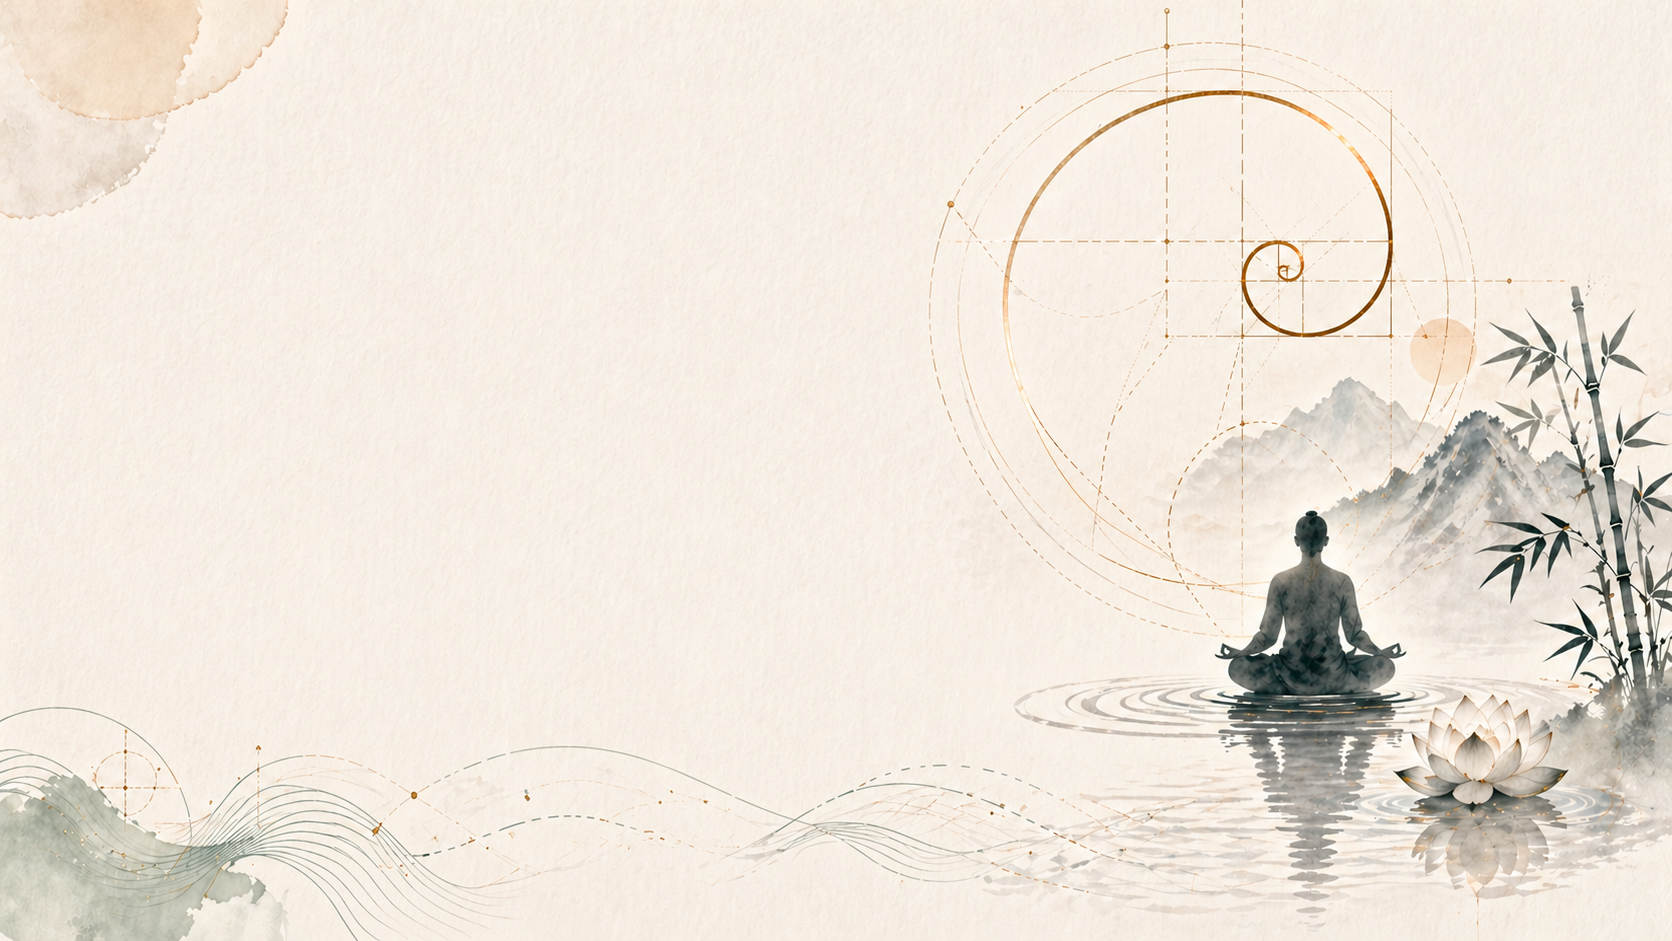
\includegraphics[width=\paperwidth,height=\paperheight,keepaspectratio=false]{chapter_02_bg_00.png}%
}
% ============================================================
% TITLE
% ============================================================
\begin{frame}
  \titlepage
  \note{
    Welcome to Chapter 2 of Principles of Mathematical Analysis. In this
    first section, we study finite, countable, and uncountable sets. This
    is the foundation for everything that follows in topology and analysis.
    We will learn how to compare the sizes of infinite sets, a surprisingly
    subtle question that leads to beautiful and sometimes counterintuitive
    results.
  }
\end{frame}
}

{
\usebackgroundtemplate{%
  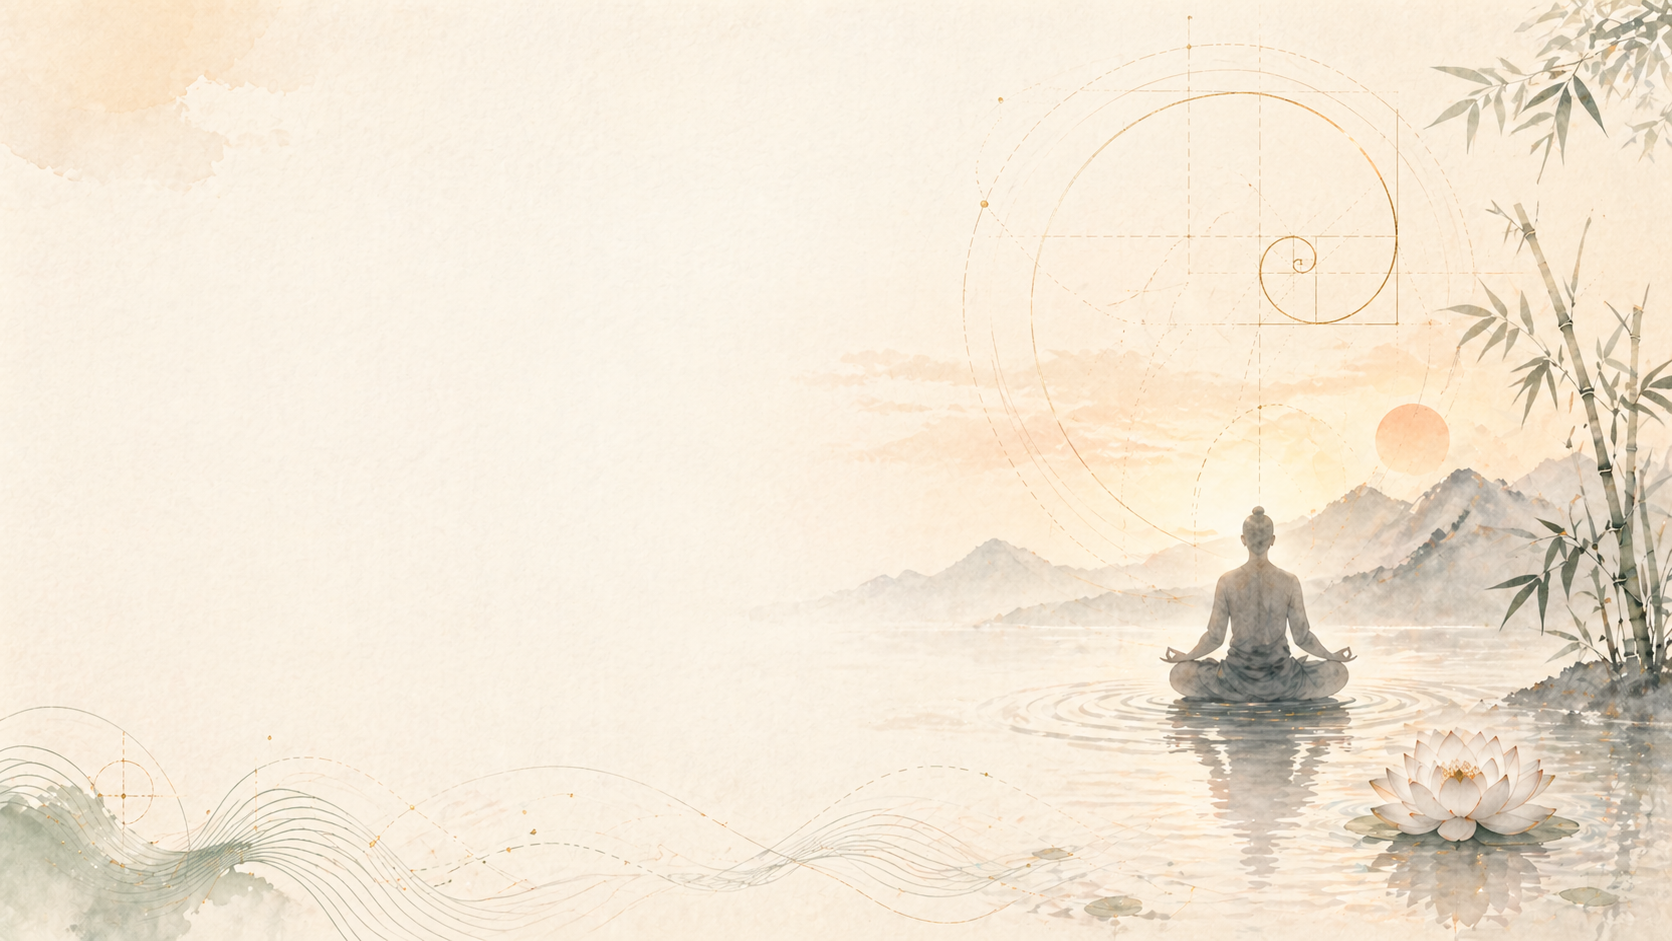
\includegraphics[width=\paperwidth,height=\paperheight,keepaspectratio=false]{chapter_02_bg_01.png}%
}
% ============================================================
% OUTLINE
% ============================================================
\begin{frame}[c]{Outline}
  \begin{center}
    \tableofcontents
  \end{center}
  \note{
    Here is what we will cover. We begin with the precise definitions of
    functions and mappings, then introduce the concept of countability,
    which lets us compare sizes of infinite sets. We will study unions and
    intersections of sets, and finally prove some powerful results about
    countability, culminating in Cantor's diagonal argument showing that
    some infinities are strictly larger than others.
  }
\end{frame}

% ============================================================
% MOTIVATION (progressive build)
% ============================================================
\section{Motivation}

% ============================================================
% --- Build 1/3 ---
\begin{frame}{Why This Section Matters}
  \begin{hlbox}
    \begin{itemize}
      \item Topology requires a precise language for \alert{sets and functions}
    \end{itemize}
  \end{hlbox}

  \note{
    Before we can study topology, which is the main subject of this chapter,
    we need a precise language for talking about sets and functions. These
    are the building blocks of all modern analysis.
  }
\end{frame}

% --- Build 2/3 ---
\begin{frame}{Why This Section Matters}
  \begin{hlbox}
    \begin{itemize}
      \item Topology requires a precise language for \alert{sets and functions}
      \item Not all infinite sets are the same ``size'' --- we need to make this precise
    \end{itemize}
  \end{hlbox}

  \note{
    A key insight in this section is that infinite sets come in different
    sizes. The integers and the rationals are both infinite, but are they
    the same kind of infinite? What about the real numbers? We need
    precise definitions to answer these questions.
  }
\end{frame}

% --- Build 3/3 ---
\begin{frame}{Why This Section Matters}
  \begin{hlbox}
    \begin{itemize}
      \item Topology requires a precise language for \alert{sets and functions}
      \item Not all infinite sets are the same ``size'' --- we need to make this precise
      \item Key tools: \emph{1-1 correspondence}, \emph{countability}, \emph{Cantor's diagonal argument}
    \end{itemize}
  \end{hlbox}

  \note{
    The main tools we develop are one-to-one correspondences for comparing
    set sizes, the notion of countability for classifying infinite sets, and
    Cantor's diagonal argument, which is one of the most elegant proofs in
    all of mathematics. Let us begin with the basics.
  }
\end{frame}
}

{
\usebackgroundtemplate{%
  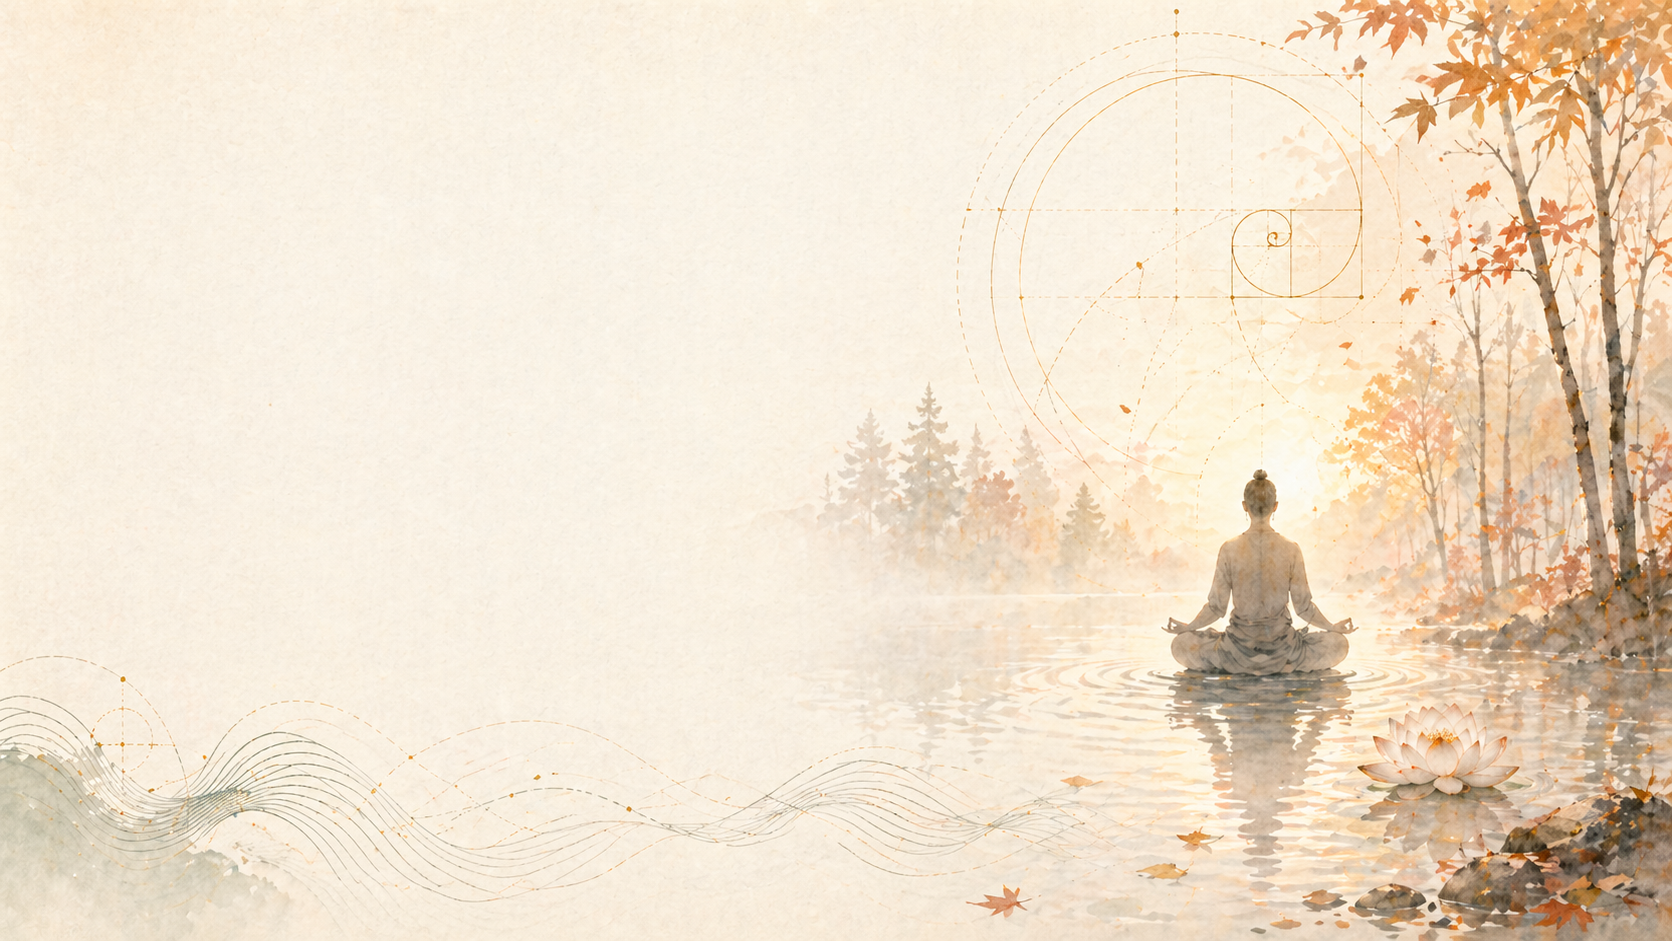
\includegraphics[width=\paperwidth,height=\paperheight,keepaspectratio=false]{chapter_02_bg_02.png}%
}
% ============================================================
\section{Functions and Mappings}

% ============================================================
\begin{frame}{Definition 2.1: Function (Mapping)}
  \begin{defblock}{Definition 2.1}
    Consider two sets $A$ and $B$. If with each element $x \in A$ there is
    associated an element of $B$, denoted $f(x)$, then $f$ is a
    \alert{function} from $A$ to $B$ (a \alert{mapping} of $A$ into $B$).

    \vspace{0.3em}
    \begin{itemize}
      \item \textbf{Domain}: the set $A$
      \item \textbf{Values}: the elements $f(x)$
      \item \textbf{Range}: the set of all values $f(A) = \{f(x) : x \in A\}$
    \end{itemize}
  \end{defblock}

  \note{
    We begin with the formal definition of a function. You may already have
    an intuitive idea of what a function is, but in analysis we need
    precision: every element of the domain must be assigned exactly one
    output. No element can be left unassigned, and no element can have two
    different outputs. Notice that the range, the set of actual outputs, may
    be smaller than "B" itself. This distinction between the range and the
    target set "B" will matter shortly. Let us look at a diagram to make
    this concrete.
  }
\end{frame}

% ============================================================
\begin{frame}{Definition 2.1: Visualizing a Function}
  \begin{center}
  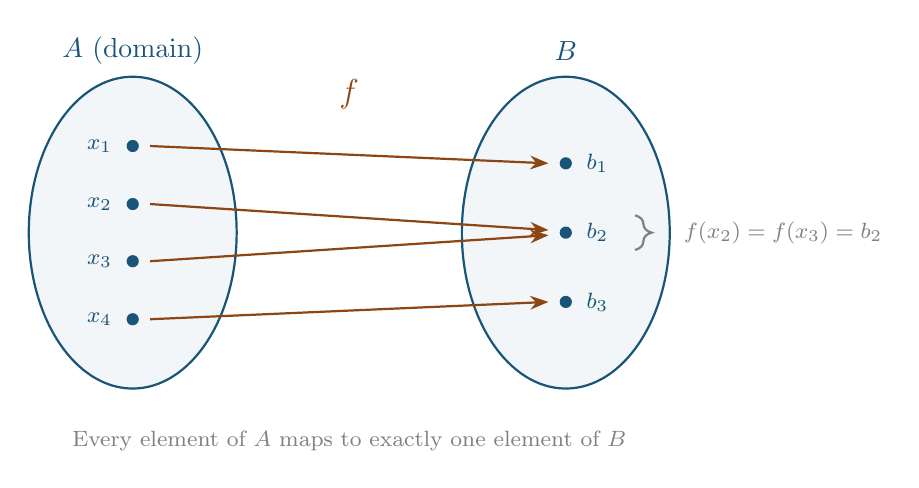
\begin{tikzpicture}[scale=1.1,
    every node/.style={font=\footnotesize},
    >=Stealth]
    % Set A
    \draw[thick, defcolor, fill=defcolor!5] (0,0) ellipse (1.2 and 1.8);
    \node[defcolor, font=\normalsize] at (0,2.1) {$A$ (domain)};
    \foreach \y/\lab in {1.0/x_1, 0.33/x_2, -0.33/x_3, -1.0/x_4} {
      \fill[defcolor] (0,\y) circle (2pt) node[left=4pt]{$\lab$};
    }
    % Set B
    \draw[thick, defcolor, fill=defcolor!5] (5,0) ellipse (1.2 and 1.8);
    \node[defcolor, font=\normalsize] at (5,2.1) {$B$};
    \foreach \y/\lab in {0.8/b_1, 0/b_2, -0.8/b_3} {
      \fill[defcolor] (5,\y) circle (2pt) node[right=4pt]{$\lab$};
    }
    % Arrows
    \draw[->,thick,mAccent] (0.2,1.0) -- (4.8,0.8);
    \draw[->,thick,mAccent] (0.2,0.33) -- (4.8,0.03);
    \draw[->,thick,mAccent] (0.2,-0.33) -- (4.8,-0.03);
    \draw[->,thick,mAccent] (0.2,-1.0) -- (4.8,-0.8);
    % Label
    \node[mAccent, font=\large] at (2.5,1.6) {$f$};
    % Annotations
    \draw[decorate, decoration={brace, amplitude=6pt, mirror}, thick, gray]
      (5.8,-0.2) -- (5.8,0.2) node[midway, right=14pt, font=\footnotesize, gray]
      {$f(x_2) = f(x_3) = b_2$};
    \node[gray, font=\footnotesize, align=left] at (2.5,-2.4)
      {Every element of $A$ maps to exactly one element of $B$};
  \end{tikzpicture}
  \end{center}

  \vspace{0.3em}
  \begin{center}
    \hl{Range $= f(A) = \{b_1, b_2, b_3\} = B$, so this $f$ maps $A$ \alert{onto} $B$.}
  \end{center}

  \note{
    Look at the diagram carefully. Notice two things. First, "x" sub 2 and
    "x" sub 3 both map to "b" sub 2. A function is allowed to send multiple
    inputs to the same output; that does not violate the definition. Second,
    every element of "B" is reached by at least one arrow, which is why this
    particular function maps "A" onto "B". If "b" sub 3 had no arrow
    pointing to it, the function would still be valid, but it would only map
    "A" into "B", not onto "B". The distinction between "into" and "onto"
    will be important when we define equivalence of sets.
  }
\end{frame}

% ============================================================
% --- Build 1/3 ---
\begin{frame}{Definition 2.2: Image, Inverse Image, 1-1 Mapping}
  \begin{defblock}{Definition 2.2 --- Image}
    If $E \subset A$, the \alert{image} of $E$ under $f$ is:
    \[
      f(E) = \{f(x) : x \in E\}
    \]
    The range of $f$ is $f(A)$. If $f(A) = B$, we say $f$ maps $A$ \alert{onto} $B$.
  \end{defblock}

  \note{
    Definition 2.2 introduces several related concepts. First, the image of
    a subset "E" of "A" is the set of all outputs you get by applying "f" to
    elements of "E". If the image of the entire domain equals "B", we say "f"
    maps "A" onto "B". Note that "onto" is stronger than "into": every element
    of "B" must actually be hit by some element of "A".
  }
\end{frame}

% --- Build 2/3 ---
\begin{frame}{Definition 2.2: Image, Inverse Image, 1-1 Mapping}
  \begin{defblock}{Definition 2.2 --- Image}
    If $E \subset A$, the \alert{image} of $E$ under $f$ is:
    \[
      f(E) = \{f(x) : x \in E\}
    \]
    The range of $f$ is $f(A)$. If $f(A) = B$, we say $f$ maps $A$ \alert{onto} $B$.
  \end{defblock}

  \begin{defblock}{Definition 2.2 --- Inverse Image}
    If $E \subset B$, the \alert{inverse image} of $E$ under $f$ is:
    \[
      f^{-1}(E) = \{x \in A : f(x) \in E\}
    \]
  \end{defblock}

  \note{
    Next, the inverse image. Given a subset "E" of "B", the inverse image
    is the set of all elements in "A" that map into "E". Note that the
    inverse image is defined even when "f" has no inverse function. It is
    simply a way of pulling subsets of "B" back to subsets of "A".
  }
\end{frame}

% --- Build 3/3 ---
\begin{frame}{Definition 2.2: Image, Inverse Image, 1-1 Mapping}
  \begin{defblock}{Definition 2.2 --- 1-1 (One-to-One) Mapping}
    $f$ is \alert{1-1} (one-to-one) if for each $y \in B$, $f^{-1}(y)$ contains
    at most one element of $A$.
    Equivalently: $f(x_1) \neq f(x_2)$ whenever $x_1 \neq x_2$.
  \end{defblock}

  \begin{center}
  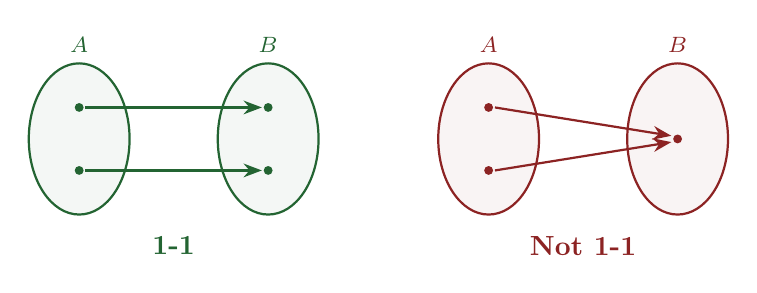
\begin{tikzpicture}[scale=0.8, every node/.style={font=\footnotesize}, >=Stealth]
    % 1-1 mapping
    \begin{scope}[xshift=0cm]
      \draw[thick, proofcolor, fill=proofcolor!5] (0,0) ellipse (0.8 and 1.2);
      \draw[thick, proofcolor, fill=proofcolor!5] (3,0) ellipse (0.8 and 1.2);
      \node[proofcolor] at (0,1.5) {$A$};
      \node[proofcolor] at (3,1.5) {$B$};
      \fill[proofcolor] (0,0.5) circle (2pt);
      \fill[proofcolor] (0,-0.5) circle (2pt);
      \fill[proofcolor] (3,0.5) circle (2pt);
      \fill[proofcolor] (3,-0.5) circle (2pt);
      \draw[->,thick,proofcolor] (0.1,0.5) -- (2.9,0.5);
      \draw[->,thick,proofcolor] (0.1,-0.5) -- (2.9,-0.5);
      \node[proofcolor, font=\normalsize] at (1.5,-1.7) {\textbf{1-1}};
    \end{scope}
    % Not 1-1 mapping
    \begin{scope}[xshift=6.5cm]
      \draw[thick, thmcolor, fill=thmcolor!5] (0,0) ellipse (0.8 and 1.2);
      \draw[thick, thmcolor, fill=thmcolor!5] (3,0) ellipse (0.8 and 1.2);
      \node[thmcolor] at (0,1.5) {$A$};
      \node[thmcolor] at (3,1.5) {$B$};
      \fill[thmcolor] (0,0.5) circle (2pt);
      \fill[thmcolor] (0,-0.5) circle (2pt);
      \fill[thmcolor] (3,0) circle (2pt);
      \draw[->,thick,thmcolor] (0.1,0.5) -- (2.9,0.05);
      \draw[->,thick,thmcolor] (0.1,-0.5) -- (2.9,-0.05);
      \node[thmcolor, font=\normalsize] at (1.5,-1.7) {\textbf{Not 1-1}};
    \end{scope}
  \end{tikzpicture}
  \end{center}

  \note{
    Why does the one-to-one property matter so much? Because it is half
    of what we need to compare the sizes of two sets. If a function is
    one-to-one, it proves that "A" is no larger than "B", since distinct
    elements of "A" use up distinct elements of "B". Combined with "onto",
    which ensures "A" is no smaller than "B", we get a perfect pairing. The
    diagram on the left shows a one-to-one mapping, while the right side
    shows a failure: two inputs collide at the same output. Next, we will
    combine both conditions to define when two sets have the same size.
  }
\end{frame}

% ============================================================
% --- Build 1/3 ---
\begin{frame}{Definition 2.3: Equivalence of Sets}
  \begin{defblock}{Definition 2.3 --- Equivalence}
    If there exists a 1-1 mapping of $A$ \alert{onto} $B$, we say $A$ and $B$:
    \begin{itemize}
      \item can be put in \alert{1-1 correspondence}
      \item have the same \alert{cardinal number}
      \item are \alert{equivalent}: $A \sim B$
    \end{itemize}
  \end{defblock}

  \note{
    This definition is the cornerstone of the entire section. Notice that
    we need both one-to-one and onto. One-to-one alone would mean "A" is
    no bigger than "B", and onto alone would mean "A" covers all of "B".
    Together they give a perfect pairing, what mathematicians call a
    bijection, and this is our precise way of saying two sets have the same
    size. The word "cardinal number" is used loosely here; a rigorous
    treatment of cardinal arithmetic requires more set theory than Rudin
    develops, but the intuition is clear: equivalent sets are the same size.
  }
\end{frame}

% --- Build 2/3 ---
\begin{frame}{Definition 2.3: Equivalence of Sets}
  \begin{defblock}{Definition 2.3 --- Equivalence}
    If there exists a 1-1 mapping of $A$ \alert{onto} $B$, we say $A$ and $B$:
    \begin{itemize}
      \item can be put in \alert{1-1 correspondence}
      \item have the same \alert{cardinal number}
      \item are \alert{equivalent}: $A \sim B$
    \end{itemize}
  \end{defblock}

  \begin{hlbox}
    This relation is an \alert{equivalence relation}:
    \begin{itemize}
      \item \textbf{Reflexive:} $A \sim A$
      \item \textbf{Symmetric:} $A \sim B \;\Rightarrow\; B \sim A$
    \end{itemize}
  \end{hlbox}

  \note{
    The equivalence relation has three properties. First, reflexivity:
    every set is equivalent to itself via the identity function. Second,
    symmetry: if "A" is equivalent to "B", then "B" is equivalent to "A",
    because we can invert a bijection.
  }
\end{frame}

% --- Build 3/3 ---
\begin{frame}{Definition 2.3: Equivalence of Sets}
  \begin{defblock}{Definition 2.3 --- Equivalence}
    If there exists a 1-1 mapping of $A$ \alert{onto} $B$, we say $A$ and $B$:
    \begin{itemize}
      \item can be put in \alert{1-1 correspondence}
      \item have the same \alert{cardinal number}
      \item are \alert{equivalent}: $A \sim B$
    \end{itemize}
  \end{defblock}

  \begin{hlbox}
    This relation is an \alert{equivalence relation}:
    \begin{itemize}
      \item \textbf{Reflexive:} $A \sim A$
      \item \textbf{Symmetric:} $A \sim B \;\Rightarrow\; B \sim A$
      \item \textbf{Transitive:} $A \sim B$ and $B \sim C \;\Rightarrow\; A \sim C$
    \end{itemize}
  \end{hlbox}

  \note{
    And third, transitivity: if "A" is equivalent to "B" and "B" is
    equivalent to "C", then "A" is equivalent to "C", because we can compose
    two bijections. Any relation satisfying these three properties is called
    an equivalence relation. Now let us use this concept to classify sets by
    their size.
  }
\end{frame}
}

{
\usebackgroundtemplate{%
  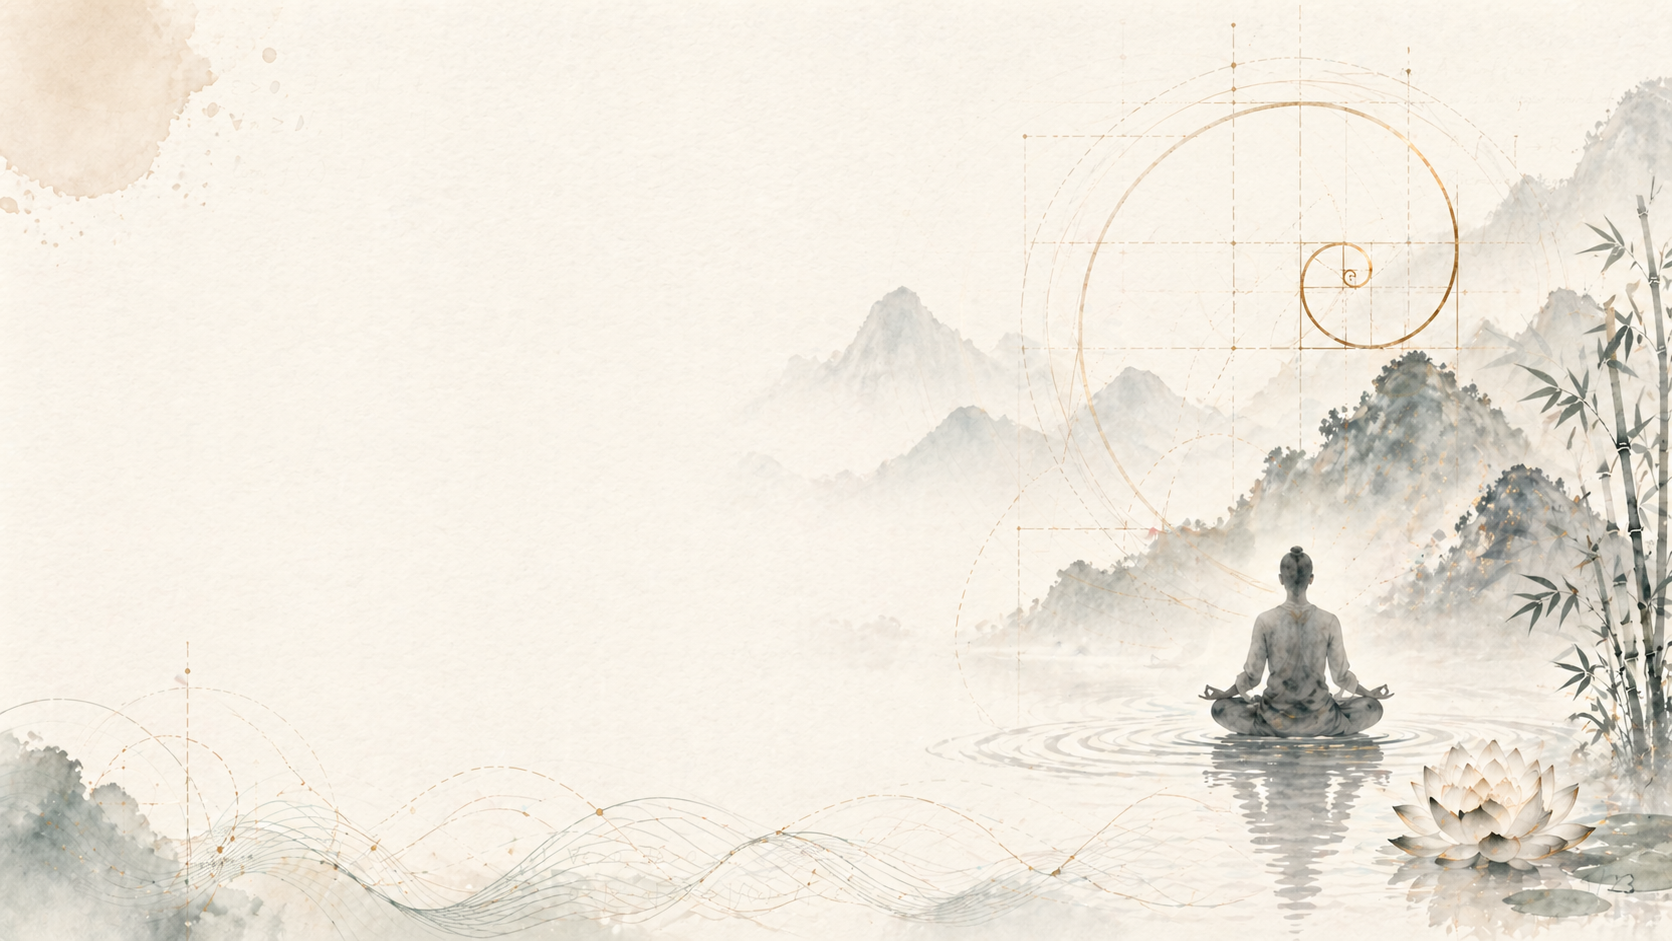
\includegraphics[width=\paperwidth,height=\paperheight,keepaspectratio=false]{chapter_02_bg_03.png}%
}
% ============================================================
\section{Countability}

% ============================================================
\begin{frame}{Definition 2.4: Finite, Countable, and Uncountable Sets}
  \begin{defblock}{Definition 2.4}
    Let $J_n = \{1, 2, \dots, n\}$ and $J = \{1, 2, 3, \dots\}$ (all positive integers).

    \vspace{0.3em}
    \begin{tabular}{@{}ll@{}}
      (a) $A$ is \alert{finite} & if $A \sim J_n$ for some $n$ (or $A = \varnothing$) \\[3pt]
      (b) $A$ is \alert{infinite} & if $A$ is not finite \\[3pt]
      (c) $A$ is \alert{countable} & if $A \sim J$ \\[3pt]
      (d) $A$ is \alert{uncountable} & if $A$ is neither finite nor countable \\[3pt]
      (e) $A$ is \alert{at most countable} & if $A$ is finite or countable
    \end{tabular}
  \end{defblock}

  \note{
    Pay attention to Rudin's terminology, because it differs from some
    other authors. For Rudin, "countable" means specifically equivalent to
    the full set of positive integers, that is, countably infinite. Some
    textbooks use "countable" to include finite sets as well. Rudin uses the
    phrase "at most countable" for that broader meaning. This distinction
    will matter in the theorems that follow. The key conceptual point is
    that we now have a hierarchy of sizes: finite sets are the smallest,
    then countable sets form the next level, and uncountable sets are
    strictly larger. Whether there are sizes between countable and
    uncountable is a deep question related to the continuum hypothesis.
  }
\end{frame}

% ============================================================
\begin{frame}{Example 2.5: The Integers Are Countable}
  \begin{exblock}{Example 2.5}
    The set $A = \mathbb{Z}$ of all integers is \alert{countable}.
  \end{exblock}

  \vspace{0.3em}
  \begin{hlbox}
    \textbf{Arrangement:}
    \begin{align*}
      A&: \quad 0,\ 1,\ {-1},\ 2,\ {-2},\ 3,\ {-3},\ \dots \\
      J&: \quad 1,\ 2,\ \phantom{-}3,\ 4,\ \phantom{-}5,\ 6,\ \phantom{-}7,\ \dots
    \end{align*}

    \textbf{Explicit formula:}
    \[
      f(n) = \begin{cases}
        \dfrac{n}{2} & \text{if } n \text{ is even}, \\[6pt]
        -\dfrac{n-1}{2} & \text{if } n \text{ is odd}.
      \end{cases}
    \]
  \end{hlbox}

  \note{
    Here is our first surprising example. The integers include both positive
    and negative numbers, so intuitively there are "twice as many" integers
    as positive integers. But they are equivalent! We can list them as
    0, 1, negative 1, 2, negative 2, 3, negative 3, and so on. The explicit
    formula shows exactly how to pair each positive integer "n" with an
    integer. Even numbers map to positive integers and odd numbers map to
    negative integers and zero. This is a perfect one-to-one correspondence.
  }
\end{frame}

% ============================================================
\begin{frame}{Example 2.5: Visualizing the Correspondence}
  \begin{center}
  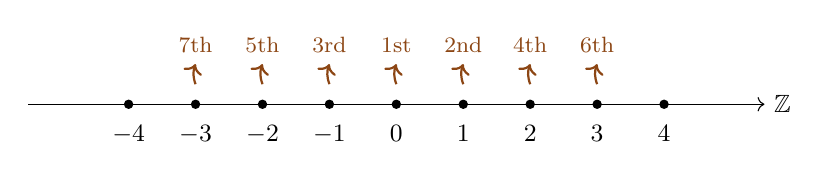
\begin{tikzpicture}[scale=0.85, every node/.style={font=\small}]
    % Number line for Z
    \draw[->] (-5.5,0) -- (5.5,0);
    \node[right] at (5.5,0) {$\mathbb{Z}$};
    \foreach \x in {-4,-3,-2,-1,0,1,2,3,4} {
      \fill (\x,0) circle (2pt);
      \node[below=4pt] at (\x,0) {$\x$};
    }
    % Arrows showing the ordering
    \draw[->,thick,mAccent] (0,0.3) to[bend left=20] ++(0,0.3);
    \node[above=8pt,mAccent,font=\footnotesize] at (0,0.3) {$1$st};
    \draw[->,thick,mAccent] (1,0.3) to[bend left=20] ++(0,0.3);
    \node[above=8pt,mAccent,font=\footnotesize] at (1,0.3) {$2$nd};
    \draw[->,thick,mAccent] (-1,0.3) to[bend left=20] ++(0,0.3);
    \node[above=8pt,mAccent,font=\footnotesize] at (-1,0.3) {$3$rd};
    \draw[->,thick,mAccent] (2,0.3) to[bend left=20] ++(0,0.3);
    \node[above=8pt,mAccent,font=\footnotesize] at (2,0.3) {$4$th};
    \draw[->,thick,mAccent] (-2,0.3) to[bend left=20] ++(0,0.3);
    \node[above=8pt,mAccent,font=\footnotesize] at (-2,0.3) {$5$th};
    \draw[->,thick,mAccent] (3,0.3) to[bend left=20] ++(0,0.3);
    \node[above=8pt,mAccent,font=\footnotesize] at (3,0.3) {$6$th};
    \draw[->,thick,mAccent] (-3,0.3) to[bend left=20] ++(0,0.3);
    \node[above=8pt,mAccent,font=\footnotesize] at (-3,0.3) {$7$th};
  \end{tikzpicture}
  \end{center}

  \vspace{0.5em}
  \begin{hlbox}
    \textbf{Key idea:} We ``zigzag'' through $\mathbb{Z}$, visiting $0$, then $\pm 1$, then $\pm 2$, \dots
  \end{hlbox}

  \note{
    The zigzag trick shown here illustrates a general principle: to prove a
    set is countable, you just need to find any systematic way to list all
    its elements as a sequence. The listing does not need to follow the
    natural order of the elements. Here, instead of trying to start from
    negative infinity, which is impossible, we start at zero and alternate
    between positive and negative integers. This idea of clever enumeration
    will appear again in the proofs of Theorems 2.12 and 2.13, where we
    use diagonal enumeration for more complex situations.
  }
\end{frame}

% ============================================================
\begin{frame}{Remark 2.6: Infinite Sets and Proper Subsets}
  \begin{remblock}{Remark 2.6}
    A \emph{finite} set cannot be equivalent to any of its proper subsets.

    \vspace{0.3em}
    However, an \emph{infinite} set \emph{can} be equivalent to a proper subset of itself!
  \end{remblock}

  \vspace{0.5em}
  \begin{hlbox}
    \textbf{Example:} $J \subset \mathbb{Z}$ is a proper subset, yet $J \sim \mathbb{Z}$ (Example 2.5).

    \vspace{0.5em}
    \textbf{Alternative definition of infinite:}\\
    $A$ is infinite $\;\iff\;$ $A$ is equivalent to one of its proper subsets.
  \end{hlbox}

  \note{
    This remark highlights a key difference between finite and infinite sets.
    If you remove an element from a finite set, you always get a strictly
    smaller set. But for infinite sets, this is not true! Example 2.5 showed
    that the positive integers are equivalent to all integers, even though
    the positive integers are a proper subset. In fact, this property can
    serve as an alternative definition of infinity: a set is infinite if and
    only if it can be put in one-to-one correspondence with a proper subset
    of itself. This is sometimes called Dedekind's definition of infinite
    sets.
  }
\end{frame}

% ============================================================
\begin{frame}{Definition 2.7: Sequences}
  \begin{defblock}{Definition 2.7}
    A \alert{sequence} is a function $f$ defined on $J = \{1, 2, 3, \dots\}$.

    \vspace{0.3em}
    If $f(n) = x_n$, we write $\{x_n\}$ or $x_1, x_2, x_3, \dots$

    \vspace{0.3em}
    The values $x_n$ are the \alert{terms} of the sequence.
  \end{defblock}

  \vspace{0.5em}
  \begin{hlbox}
    \textbf{Key observations:}
    \begin{itemize}
      \item Terms need \emph{not} be distinct
      \item Every countable set is the range of a sequence of \emph{distinct} terms
      \item We can ``arrange'' any countable set in a sequence
    \end{itemize}
  \end{hlbox}

  \note{
    The formal definition of a sequence as a function on the positive
    integers may seem overly pedantic, but it is important. It lets us
    apply function concepts like range and one-to-one to sequences.
    The crucial observation is the link between sequences and countability:
    saying a set is countable is the same as saying its elements can be
    arranged as a sequence of distinct terms. This is why "countable" is
    sometimes called "enumerable." Conversely, a sequence whose terms are
    not all distinct has a range that is at most countable, not necessarily
    countable. We will rely on this connection in the very next theorem.
  }
\end{frame}

% ============================================================
\begin{frame}{Theorem 2.8: Infinite Subsets of Countable Sets}
  \begin{thmblock}{Theorem 2.8}
    Every infinite subset of a countable set $A$ is countable.
  \end{thmblock}

  \vspace{0.5em}
  \begin{hlbox}
    \textbf{Consequence:} Countable sets are the ``smallest'' infinity.

    No uncountable set can be a subset of a countable set.
  \end{hlbox}

  \note{
    This theorem establishes that countable infinity is the smallest type
    of infinity. You might wonder: could there be an infinite set that is
    too small to be countable? This theorem says no. Every infinite subset
    of a countable set is itself countable. So there is nothing between
    finite and countable. This fact will be used as a workhorse throughout
    the section: whenever we need to show a set is countable, it often
    suffices to embed it into a known countable set and verify it is
    infinite. Let us see the proof.
  }
\end{frame}

% ============================================================
\begin{frame}{Proof of Theorem 2.8 --- Strategy}
  \begin{proofblock}{Proof Strategy}
    \textbf{Given:} $E \subset A$, $A$ countable, $E$ infinite.

    \textbf{Goal:} Show $E \sim J$ (i.e., $E$ is countable).

    \vspace{0.3em}
    \textbf{Approach:}
    \begin{enumerate}
      \item Arrange $A$ in a sequence $\{x_n\}$ of distinct terms.
      \item Pick out the elements of $E$ \emph{in order of their indices}.
      \item This gives a 1-1 correspondence between $E$ and $J$.
    \end{enumerate}
  \end{proofblock}

  \note{
    The idea behind the proof is to inherit the ordering from "A". Since
    "A" is countable, it already comes with a sequence ordering. We simply
    filter this sequence, keeping only elements of "E". The key subtlety
    is why this produces a bijection with the positive integers: the
    one-to-one property follows because we pick each element at most once,
    and the onto property follows because "E" is infinite, so the filtering
    process never terminates. If "E" were finite, we would run out of
    elements and only get a bijection with some finite set.
  }
\end{frame}

% --- Proof Step 1 ---
\begin{frame}{Proof of Theorem 2.8 --- Construction}
  \begin{proofblock}{Step 1: Set up the subsequence}
    Arrange $A = \{x_1, x_2, x_3, \dots\}$ (distinct terms).

    \vspace{0.3em}
    Construct a sequence of indices $\{n_k\}$:
    \begin{itemize}
      \item $n_1 =$ smallest index with $x_{n_1} \in E$
      \item $n_k =$ smallest index $> n_{k-1}$ with $x_{n_k} \in E$
    \end{itemize}
  \end{proofblock}

  \begin{proofblock}{Step 2: Conclude}
    Define $f(k) = x_{n_k}$.

    Then $f$ is a 1-1 correspondence between $J$ and $E$. \qed
  \end{proofblock}

  \note{
    Here is the construction. We start with "A" listed as a sequence. To
    find the first element of "E", we scan through the sequence and take the
    first element that belongs to "E". Call its index "n" sub 1. For the
    second element, we continue scanning past index "n" sub 1 and take the
    next element in "E", and so on. Since "E" is infinite, this process
    never terminates. The function "f" of "k" equals "x" sub "n" sub "k"
    gives us a one-to-one correspondence between the positive integers and
    "E". The proof is complete.
  }
\end{frame}
}

{
\usebackgroundtemplate{%
  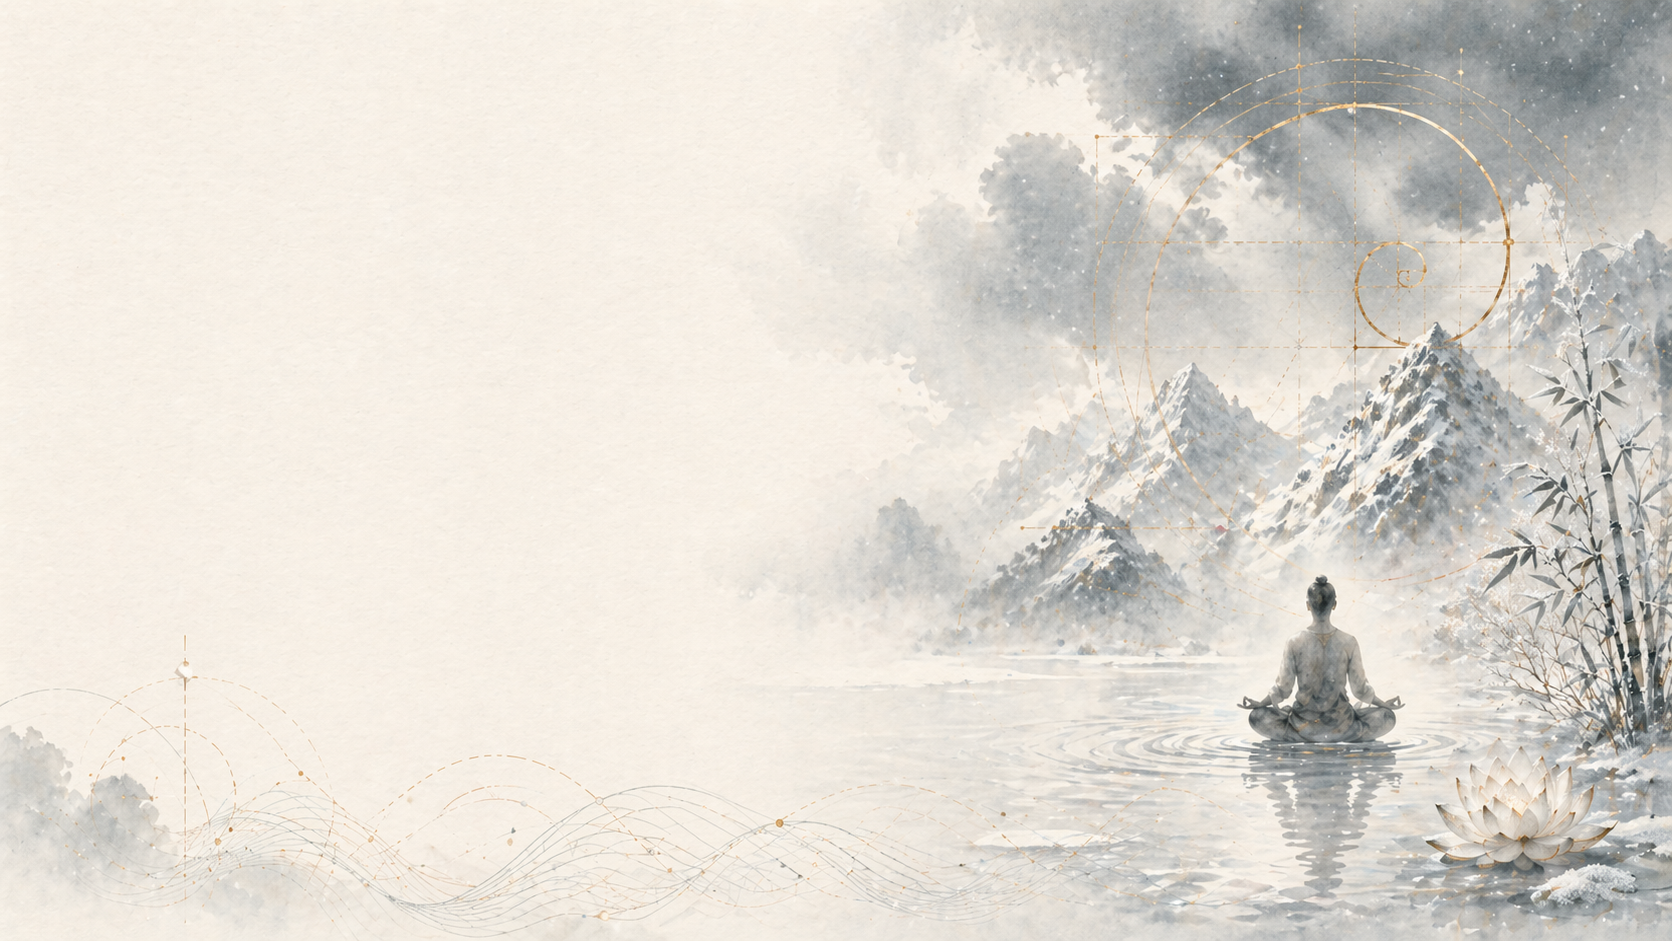
\includegraphics[width=\paperwidth,height=\paperheight,keepaspectratio=false]{chapter_02_bg_04.png}%
}
% ============================================================
\section{Unions and Intersections}

% ============================================================
% --- Build 1/2 ---
\begin{frame}{Definition 2.9: Union and Intersection}
  \begin{defblock}{Definition 2.9 --- Union}
    Given a family of sets $\{E_\alpha\}$ indexed by $A$, the \alert{union} is:
    \[
      S = \bigcup_{\alpha \in A} E_\alpha
      = \{x : x \in E_\alpha \text{ for at least one } \alpha \in A\}
    \]

    Special cases:
    $\displaystyle\bigcup_{m=1}^{n} E_m = E_1 \cup \cdots \cup E_n$
    \qquad
    $\displaystyle\bigcup_{m=1}^{\infty} E_m$
  \end{defblock}

  \note{
    Why does Rudin define unions and intersections so generally, using an
    arbitrary index set "A"? Because in topology and analysis, we
    frequently need unions over uncountable families, not just finite or
    countable ones. For example, when we later define open sets, we will
    need to take unions of uncountably many neighborhoods. The general
    notation with a subscript "alpha" in "A" handles all cases uniformly.
    The special cases shown at the bottom are just convenient shorthand for
    finite and countable unions.
  }
\end{frame}

% --- Build 2/2 ---
\begin{frame}{Definition 2.9: Union and Intersection}
  \begin{defblock}{Definition 2.9 --- Union}
    $\displaystyle S = \bigcup_{\alpha \in A} E_\alpha
      = \{x : x \in E_\alpha \text{ for at least one } \alpha \in A\}$
  \end{defblock}

  \begin{defblock}{Definition 2.9 --- Intersection}
    $\displaystyle P = \bigcap_{\alpha \in A} E_\alpha
      = \{x : x \in E_\alpha \text{ for every } \alpha \in A\}$
  \end{defblock}

  \vspace{0.5em}
  \begin{hlbox}
    If $A \cap B \neq \varnothing$, we say $A$ and $B$ \alert{intersect}; otherwise they are \alert{disjoint}.
  \end{hlbox}

  \note{
    Notice the contrast: for the union, an element needs to be in just one
    of the sets, while for the intersection, it must be in every single
    one. As we will see in Example 2.10, this makes intersections of
    infinite families much more restrictive and sometimes empty even when
    every individual set is nonempty. The terminology "disjoint" for
    non-intersecting sets will appear constantly in topology, particularly
    when we discuss separation properties and partitions. Let us look at
    some concrete examples.
  }
\end{frame}

% ============================================================
\begin{frame}{Examples 2.10: Union and Intersection}
  \begin{exblock}{Example 2.10(a)}
    $E_1 = \{1, 2, 3\}$, \quad $E_2 = \{2, 3, 4\}$

    $E_1 \cup E_2 = \{1, 2, 3, 4\}$, \quad $E_1 \cap E_2 = \{2, 3\}$
  \end{exblock}

  \begin{center}
  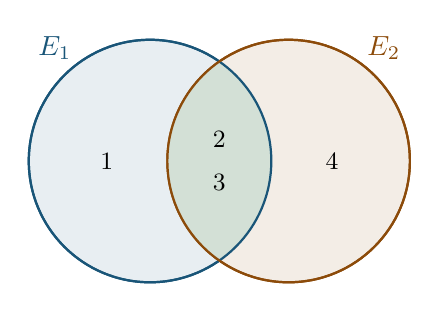
\begin{tikzpicture}[scale=1.1, every node/.style={font=\small}]
    % E1 circle
    \fill[defcolor!10] (0,0) circle (1.4);
    \draw[thick, defcolor] (0,0) circle (1.4);
    % E2 circle
    \fill[excolor!10] (1.6,0) circle (1.4);
    \draw[thick, excolor] (1.6,0) circle (1.4);
    % Intersection shading (drawn after circles, then redraw borders on top)
    \begin{scope}
      \clip (0,0) circle (1.4);
      \fill[proofcolor!20] (1.6,0) circle (1.4);
    \end{scope}
    % Redraw borders on top so they are fully visible
    \draw[thick, defcolor] (0,0) circle (1.4);
    \draw[thick, excolor] (1.6,0) circle (1.4);
    % Set labels (outside circles)
    \node[defcolor, font=\normalsize\bfseries] at (-1.1,1.3) {$E_1$};
    \node[excolor, font=\normalsize\bfseries] at (2.7,1.3) {$E_2$};
    % Element labels
    \node at (-0.5,0) {$1$};
    \node at (0.8,0.25) {$2$};
    \node at (0.8,-0.25) {$3$};
    \node at (2.1,0) {$4$};
  \end{tikzpicture}
  \end{center}

  \note{
    This is a straightforward example with finite sets, where union and
    intersection behave exactly as you would expect. The green overlap in
    the Venn diagram is the intersection. Notice that the union has 4
    elements, not 6: we do not count 2 and 3 twice. In general, for
    finite sets, the size of "A" union "B" equals the size of "A" plus the
    size of "B" minus the size of "A" intersect "B". This inclusion-
    exclusion principle generalizes to more than two sets. The next example
    is more subtle, involving an uncountable family of sets.
  }
\end{frame}

% ============================================================
% --- Build 1/3 ---
\begin{frame}{Example 2.10(b): A Continuous Family of Sets}
  \begin{exblock}{Example 2.10(b)}
    For each $x \in (0, 1]$, let $E_x = \{y \in \mathbb{R} : 0 < y < x\} = (0, x)$.
  \end{exblock}

  \vspace{0.3em}
  \begin{hlbox}
    (i) $E_x \subset E_z$ if and only if $0 < x \leq z \leq 1$
  \end{hlbox}

  \note{
    Part "b" is more interesting. Here we have a continuous family of sets
    indexed by the interval from 0 to 1. Each set "E" sub "x" is the open
    interval from 0 to "x". The containment relation is natural: a smaller
    "x" gives a smaller interval.
  }
\end{frame}

% --- Build 2/3 ---
\begin{frame}{Example 2.10(b): A Continuous Family of Sets}
  \begin{exblock}{Example 2.10(b)}
    For each $x \in (0, 1]$, let $E_x = \{y \in \mathbb{R} : 0 < y < x\} = (0, x)$.
  \end{exblock}

  \vspace{0.3em}
  \begin{hlbox}
    (i) $E_x \subset E_z$ if and only if $0 < x \leq z \leq 1$

    \vspace{0.3em}
    (ii) $\displaystyle\bigcup_{x \in (0,1]} E_x = E_1 = (0, 1)$
  \end{hlbox}

  \note{
    The union of all these intervals is the largest one, which is the open
    interval from 0 to 1. This makes sense because "E" sub 1 contains all
    the others, so their union is just "E" sub 1 itself.
  }
\end{frame}

% --- Build 3/3 ---
\begin{frame}{Example 2.10(b): A Continuous Family of Sets}
  \begin{exblock}{Example 2.10(b)}
    For each $x \in (0, 1]$, let $E_x = \{y \in \mathbb{R} : 0 < y < x\} = (0, x)$.
  \end{exblock}

  \vspace{0.3em}
  \begin{hlbox}
    (i) $E_x \subset E_z$ if and only if $0 < x \leq z \leq 1$

    \vspace{0.3em}
    (ii) $\displaystyle\bigcup_{x \in (0,1]} E_x = E_1 = (0, 1)$

    \vspace{0.3em}
    (iii) $\displaystyle\bigcap_{x \in (0,1]} E_x = \varnothing$

    \vspace{0.3em}
    \emph{Why?} For any $y > 0$, if $x < y$ then $y \notin E_x$.
    So no $y$ belongs to \emph{every} $E_x$.
  \end{hlbox}

  \note{
    The intersection is empty! This is the surprising part. For any positive
    number "y", no matter how small, we can find an "x" less than "y", and
    then "y" does not belong to "E" sub "x". So no single "y" is in all the
    sets simultaneously. This shows that intersections of infinitely many
    sets can behave very differently from finite intersections.
  }
\end{frame}

% ============================================================
% --- Build 1/4 ---
\begin{frame}{Remarks 2.11: Algebraic Properties of Set Operations}
  \begin{hlbox}
    \textbf{Commutative laws:}
    \[
      A \cup B = B \cup A; \qquad A \cap B = B \cap A.
    \]
  \end{hlbox}

  \note{
    Rudin lists several algebraic properties of unions and intersections that
    are analogous to properties of addition and multiplication. First, the
    commutative laws: the order does not matter for either union or
    intersection.
  }
\end{frame}

% --- Build 2/4 ---
\begin{frame}{Remarks 2.11: Algebraic Properties of Set Operations}
  \begin{hlbox}
    \textbf{Commutative laws:}
    \[
      A \cup B = B \cup A; \qquad A \cap B = B \cap A.
    \]

    \textbf{Associative laws:}
    \[
      (A \cup B) \cup C = A \cup (B \cup C); \qquad
      (A \cap B) \cap C = A \cap (B \cap C).
    \]
  \end{hlbox}

  \note{
    The associative laws say that grouping does not matter. We can write
    "A" union "B" union "C" without ambiguity. The same holds for
    intersection.
  }
\end{frame}

% --- Build 3/4 ---
\begin{frame}{Remarks 2.11: Algebraic Properties of Set Operations}
  \begin{hlbox}
    \textbf{Commutative laws:}
    \[
      A \cup B = B \cup A; \qquad A \cap B = B \cap A.
    \]

    \textbf{Associative laws:}
    \[
      (A \cup B) \cup C = A \cup (B \cup C); \qquad
      (A \cap B) \cap C = A \cap (B \cap C).
    \]

    \textbf{Distributive law:}
    \[
      \boxed{A \cap (B \cup C) = (A \cap B) \cup (A \cap C)}
    \]
  \end{hlbox}

  \note{
    The distributive law is the most important one. Intersection distributes
    over union, just as multiplication distributes over addition. The proof
    is a straightforward element-chasing argument: you show that every
    element of the left side belongs to the right side, and vice versa.
  }
\end{frame}

% --- Build 4/4 ---
\begin{frame}{Remarks 2.11: Algebraic Properties of Set Operations}
  \begin{hlbox}
    \textbf{Further identities} (with $\varnothing$ denoting the empty set):
    \begin{align*}
      &A \subset A \cup B, \qquad A \cap B \subset A \\[4pt]
      &A \cup \varnothing = A, \qquad A \cap \varnothing = \varnothing \\[4pt]
      &\text{If } A \subset B: \\[4pt]
      &A \cup B = B, \qquad A \cap B = A
    \end{align*}
  \end{hlbox}

  \note{
    Rudin also lists several additional identities. "A" is always a subset
    of "A" union "B", and "A" intersect "B" is always a subset of "A". The
    empty set acts as an identity for union and as an annihilator for
    intersection. And if "A" is a subset of "B", then their union is just
    "B" and their intersection is just "A". These properties are easy to
    verify directly from the definitions. Now let us move to the main
    countability results of this section.
  }
\end{frame}
}

{
\usebackgroundtemplate{%
  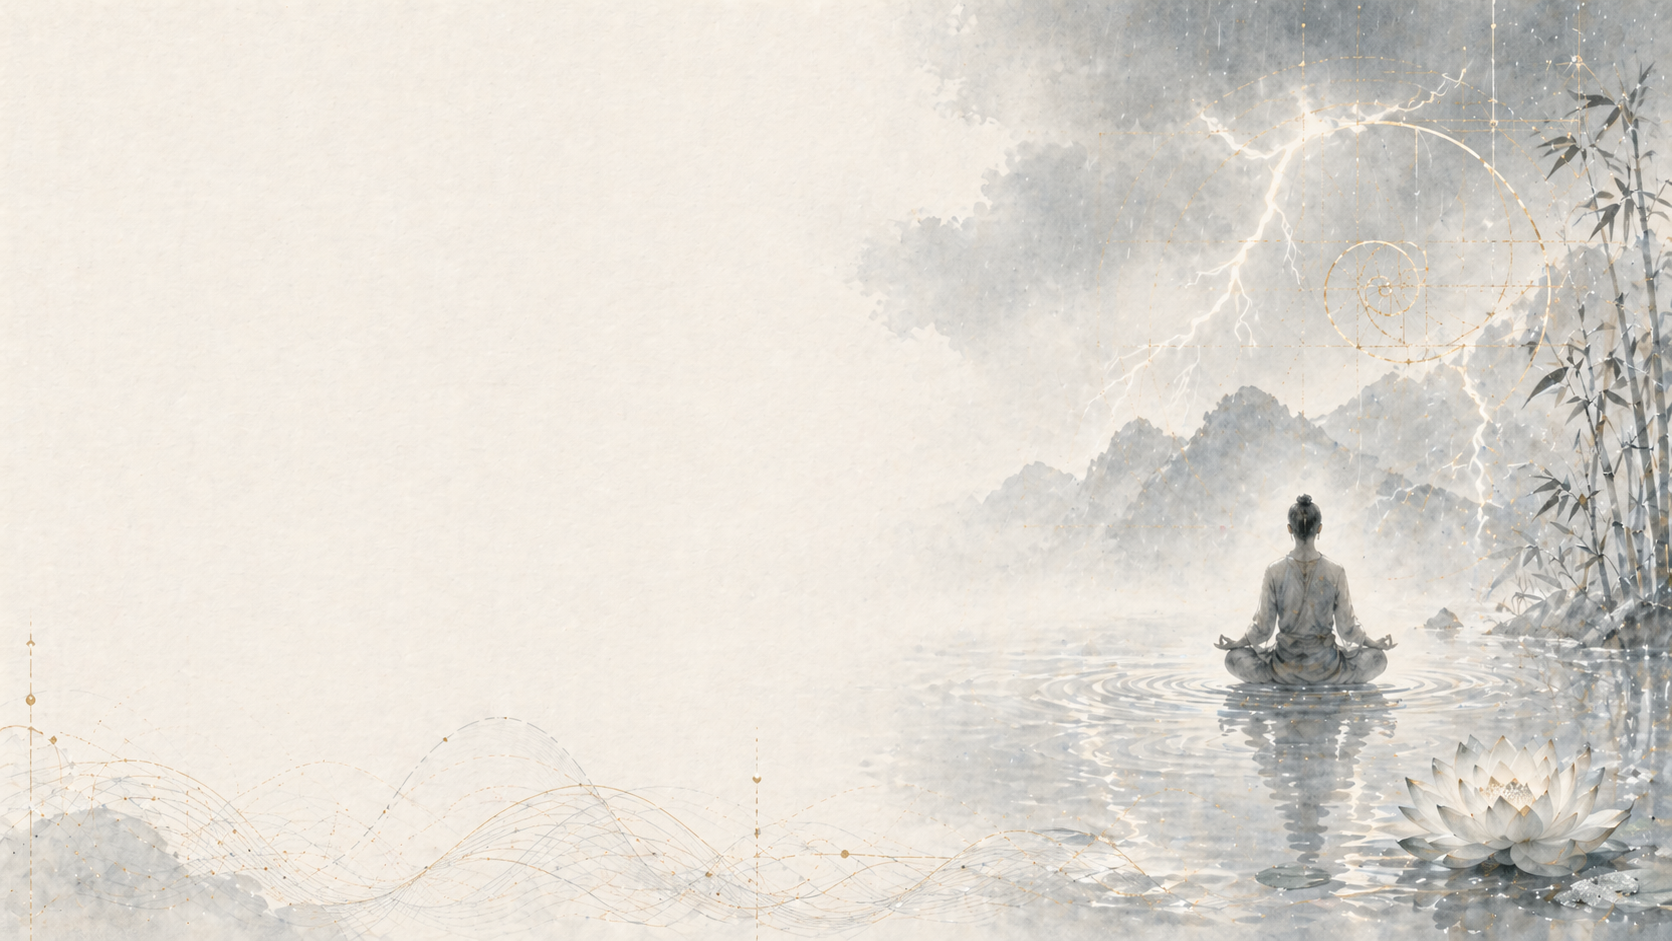
\includegraphics[width=\paperwidth,height=\paperheight,keepaspectratio=false]{chapter_02_bg_05.png}%
}
% ============================================================
\section{Countability Results}

% ============================================================
\begin{frame}{Theorem 2.12: Countable Union of Countable Sets}
  \begin{thmblock}{Theorem 2.12}
    Let $\{E_n\}$, $n = 1, 2, 3, \dots$, be a sequence of countable sets, and put
    \[
      S = \bigcup_{n=1}^{\infty} E_n.
    \]
    Then $S$ is countable.
  \end{thmblock}

  \vspace{0.5em}
  \begin{center}
    \hl{\textbf{In words:} A countable union of countable sets is countable.}
  \end{center}

  \note{
    This is one of the most powerful results in this section. It says that
    if you take countably many sets, each of which is countable, and form
    their union, the result is still countable. You might think that
    combining countably many infinite sets would produce something
    uncountable, but it does not. The proof uses a beautiful diagonal
    arrangement.
  }
\end{frame}

% ============================================================
\begin{frame}{Proof of Theorem 2.12 --- The Diagonal Arrangement}
  \begin{proofblock}{Step 1: Arrange each $E_n$ as a sequence}
    Write $E_n = \{x_{n1}, x_{n2}, x_{n3}, \dots\}$ and form the array:
  \end{proofblock}

  \begin{center}
  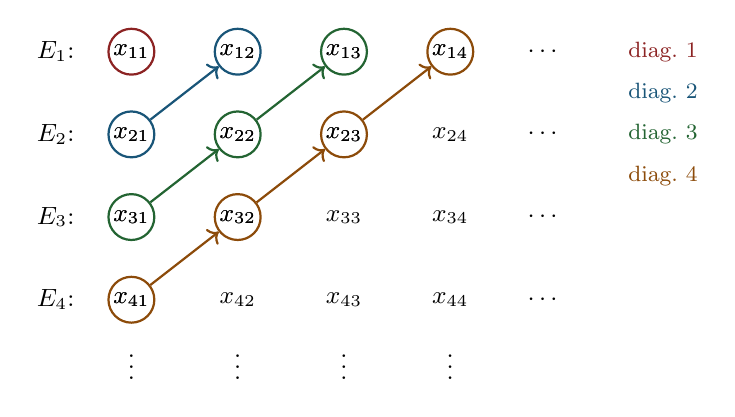
\begin{tikzpicture}[scale=0.75, every node/.style={font=\small}]
    % Grid of elements (named nodes for precise arrow placement)
    \foreach \r/\rlab in {0/1, -1.4/2, -2.8/3, -4.2/4} {
      \node[left] at (-0.8,\r) {$E_{\rlab}$:};
    }
    \foreach \r/\rn/\ri in {0/1/1, -1.4/2/2, -2.8/3/3, -4.2/4/4} {
      \foreach \c/\cn/\ci in {0/1/1, 1.8/2/2, 3.6/3/3, 5.4/4/4} {
        \node (n\ri\ci) at (\c,\r) {$x_{\rn\cn}$};
      }
      \node at (7,\r) {$\cdots$};
    }
    \node at (0,-5.2) {$\vdots$};
    \node at (1.8,-5.2) {$\vdots$};
    \node at (3.6,-5.2) {$\vdots$};
    \node at (5.4,-5.2) {$\vdots$};
    % Color-coded diagonal circles (named for arrow connections)
    \node[circle, draw=thmcolor, thick, inner sep=1pt] (d11) at (0,0) {$x_{11}$};
    \node[circle, draw=defcolor, thick, inner sep=1pt] (d21) at (0,-1.4) {$x_{21}$};
    \node[circle, draw=defcolor, thick, inner sep=1pt] (d12) at (1.8,0) {$x_{12}$};
    \node[circle, draw=proofcolor, thick, inner sep=1pt] (d31) at (0,-2.8) {$x_{31}$};
    \node[circle, draw=proofcolor, thick, inner sep=1pt] (d22) at (1.8,-1.4) {$x_{22}$};
    \node[circle, draw=proofcolor, thick, inner sep=1pt] (d13) at (3.6,0) {$x_{13}$};
    \node[circle, draw=excolor, thick, inner sep=1pt] (d41) at (0,-4.2) {$x_{41}$};
    \node[circle, draw=excolor, thick, inner sep=1pt] (d32) at (1.8,-2.8) {$x_{32}$};
    \node[circle, draw=excolor, thick, inner sep=1pt] (d23) at (3.6,-1.4) {$x_{23}$};
    \node[circle, draw=excolor, thick, inner sep=1pt] (d14) at (5.4,0) {$x_{14}$};
    % Diagonal arrows connecting circled elements within each diagonal
    \draw[->,thick,defcolor] (d21) -- (d12);
    \draw[->,thick,proofcolor] (d31) -- (d22);
    \draw[->,thick,proofcolor] (d22) -- (d13);
    \draw[->,thick,excolor] (d41) -- (d32);
    \draw[->,thick,excolor] (d32) -- (d23);
    \draw[->,thick,excolor] (d23) -- (d14);
    % Diagonal labels
    \node[thmcolor, font=\footnotesize] at (9,0) {diag.\ 1};
    \node[defcolor, font=\footnotesize] at (9,-0.7) {diag.\ 2};
    \node[proofcolor, font=\footnotesize] at (9,-1.4) {diag.\ 3};
    \node[excolor, font=\footnotesize] at (9,-2.1) {diag.\ 4};
  \end{tikzpicture}
  \end{center}

  \note{
    The trick here is to flatten a two-dimensional array into a single
    sequence. We cannot go row by row, because we would spend all of
    eternity on just the first row and never reach the second. Instead,
    we traverse along finite diagonals: the "k"-th diagonal contains all
    entries where the row number plus the column number equals "k" plus 1.
    Each diagonal is finite, so we finish it and move on. This guarantees
    that every entry in the array is eventually reached. The color-coded
    circles on the slide show the first four diagonals. This diagonal
    enumeration idea is one of the most useful techniques in set theory.
  }
\end{frame}

% ============================================================
\begin{frame}{Proof of Theorem 2.12 --- The Diagonal Sequence}
  \begin{proofblock}{Step 2: Enumerate along diagonals}
    List the elements in order:
    \[
      x_{11};\; x_{21}, x_{12};\; x_{31}, x_{22}, x_{13};\; x_{41}, x_{32}, x_{23}, x_{14};\; \dots
    \]
  \end{proofblock}

  \begin{proofblock}{Step 3: Handle duplicates and conclude}
    \begin{itemize}
      \item If sets $E_n$ overlap, some elements repeat $\Rightarrow$ $S \sim T \subset J$
      \item By Theorem 2.8, $S$ is at most countable
      \item Since $E_1 \subset S$ and $E_1$ is infinite, $S$ is infinite
      \item Therefore $S$ is countable \qed
    \end{itemize}
  \end{proofblock}

  \note{
    There is a subtle point about duplicates. The diagonal listing may
    contain the same element more than once if the sets "E" sub "n" overlap.
    But that does not cause a problem: we simply remove repeated entries.
    Formally, this means "S" is equivalent to some subset "T" of the
    positive integers. By Theorem 2.8, "S" is at most countable. The final
    step is clever: we use the assumption that each "E" sub "n" is infinite,
    not just nonempty, so "S" contains the infinite set "E" sub 1. This
    forces "S" to be infinite, and an infinite set that is at most countable
    must be countable.
  }
\end{frame}

% ============================================================
\begin{frame}{Corollary of Theorem 2.12}
  \begin{thmblock}{Corollary}
    If $A$ is at most countable and each $B_\alpha$ (for $\alpha \in A$) is at most
    countable, then
    \[
      T = \bigcup_{\alpha \in A} B_\alpha
    \]
    is at most countable.
  \end{thmblock}

  \vspace{0.5em}
  \begin{center}
    \hl{\emph{Proof:} $T$ is equivalent to a subset of the array from Theorem 2.12.}
  \end{center}

  \note{
    This corollary relaxes the hypotheses: the index set and the individual
    sets only need to be at most countable, not necessarily countable. The
    conclusion weakens accordingly to "at most countable." This version is
    often more convenient in practice because we do not need to check
    whether the sets are finite or countable. Notice that the conclusion
    cannot be strengthened to "countable," because a finite union of finite
    sets is finite. Now let us see a powerful application of Theorem 2.12.
  }
\end{frame}

% ============================================================
\begin{frame}{Theorem 2.13: Countability of $n$-Tuples}
  \begin{thmblock}{Theorem 2.13}
    Let $A$ be a countable set, and let $B_n$ be the set of all $n$-tuples
    $(a_1, \dots, a_n)$ with $a_k \in A$. Then $B_n$ is countable.
  \end{thmblock}

  \note{
    This theorem is surprisingly powerful. It says that forming all ordered
    tuples of any fixed length from a countable set does not increase the
    size beyond countable. Think about what this means for pairs: the set of
    all pairs of integers is countable, even though it seems to be a
    "two-dimensional infinity." The key constraint is that "n" must be
    fixed. If we allowed tuples of all lengths simultaneously, we would get
    the set of all finite sequences, which is still countable, but infinite
    sequences form an uncountable set, as we will soon see.
  }
\end{frame}

% ============================================================
% --- Build 1/3 ---
\begin{frame}{Proof of Theorem 2.13}
  \begin{proofblock}{Proof by induction on $n$}
    \textbf{Base case:} $B_1 = A$ is countable.  \end{proofblock}

  \note{
    The proof uses induction on the tuple length "n". The base case is
    immediate: 1-tuples are just individual elements, so "B" sub 1 is
    simply "A" itself. The real work happens in the inductive step, where
    we reduce "n"-tuples to "n" minus 1 tuples plus one extra element.
  }
\end{frame}

% --- Build 2/3 ---
\begin{frame}{Proof of Theorem 2.13}
  \begin{proofblock}{Proof by induction on $n$}
    \textbf{Base case:} $B_1 = A$ is countable.

    \textbf{Inductive step:} Assume $B_{n-1}$ is countable.

    Elements of $B_n$ have the form $(b, a)$ where $b \in B_{n-1}$, $a \in A$.
  \end{proofblock}

  \note{
    Here is the clever decomposition. An "n"-tuple is just an "n" minus 1
    tuple with one more element appended. So we can think of "B" sub "n"
    as a collection of pairs, where the first component comes from "B" sub
    "n" minus 1 and the second comes from "A". This reduces the problem
    to understanding the set of all such pairs.
  }
\end{frame}

% --- Build 3/3 ---
\begin{frame}{Proof of Theorem 2.13}
  \begin{proofblock}{Proof by induction on $n$}
    \textbf{Base case:} $B_1 = A$ is countable.

    \textbf{Inductive step:} Assume $B_{n-1}$ is countable.

    Elements of $B_n$ have the form $(b, a)$ where $b \in B_{n-1}$, $a \in A$.

    \vspace{0.3em}
    For each fixed $b$, the set $\{(b, a) : a \in A\} \sim A$ is countable.

    $\Rightarrow$ $B_n$ is a \emph{countable union of countable sets}.

    $\Rightarrow$ $B_n$ is countable by Theorem 2.12. \qed
  \end{proofblock}

  \note{
    Now we see why Theorem 2.12 is so useful. For each fixed "b", varying
    "a" over "A" gives a countable set. And we are taking the union over
    all "b" in "B" sub "n" minus 1, which is countable by the inductive
    hypothesis. So "B" sub "n" is a countable union of countable sets.
    Theorem 2.12 immediately tells us it is countable. Notice how the
    induction and Theorem 2.12 work hand in hand: each step peels off one
    component of the tuple.
  }
\end{frame}

% ============================================================
\begin{frame}{Corollary: The Rationals Are Countable}
  \begin{thmblock}{Corollary of Theorem 2.13}
    The set $\mathbb{Q}$ of all rational numbers is \alert{countable}.
  \end{thmblock}

  \vspace{0.3em}
  \begin{proofblock}{Proof}
    Every rational $r = b/a$ where $a, b \in \mathbb{Z}$.

    The set of pairs $(a, b)$ is $B_2$ with $A = \mathbb{Z}$ (countable by Example 2.5).

    By Theorem 2.13, $B_2$ is countable.

    Since $\mathbb{Q} \sim T \subset B_2$, $\mathbb{Q}$ is at most countable.

    Since $\mathbb{Q}$ is infinite, $\mathbb{Q}$ is countable. \qed
  \end{proofblock}

  \note{
    Here is a beautiful application. Every rational number can be written
    as "b" over "a" where "a" and "b" are integers. So the rationals
    correspond to a subset of all pairs of integers. By Example 2.5, the
    integers are countable, so by Theorem 2.13, the set of all pairs is
    countable. The rationals form a subset, so by Theorem 2.8, they are at
    most countable. Since they are clearly infinite, they are countable.
    Rudin also notes that even the algebraic numbers are countable. But as
    we are about to see, not all infinite sets are countable.
  }
\end{frame}

% ============================================================
\begin{frame}{Theorem 2.14: An Uncountable Set}
  \begin{thmblock}{Theorem 2.14}
    Let $A$ be the set of all sequences whose elements are the digits $0$ and $1$.
    Then $A$ is \alert{uncountable}.
  \end{thmblock}

  \vspace{0.5em}
  \begin{hlbox}
    \textbf{Elements of $A$:}\quad sequences like $1, 0, 0, 1, 0, 1, 1, 1, \dots$

    \vspace{0.5em}
    \textbf{Technique:} \alert{Cantor's diagonal argument}
  \end{hlbox}

  \note{
    This is perhaps the most famous theorem in set theory. The set of all
    infinite binary sequences is uncountable. This is proved using Cantor's
    diagonal argument, one of the most celebrated proofs in mathematics.
    The idea is beautifully simple, yet its consequences are profound. It
    shows that some infinities are strictly larger than others.
  }
\end{frame}

% ============================================================
% --- Build 1/3 ---
\begin{frame}{Proof of Theorem 2.14 --- Cantor's Diagonal Argument}
  \begin{proofblock}{Step 1: Assume $E$ is a countable subset of $A$}
    List the elements of $E$ as sequences $s_1, s_2, s_3, \dots$:
  \end{proofblock}

  \begin{center}
  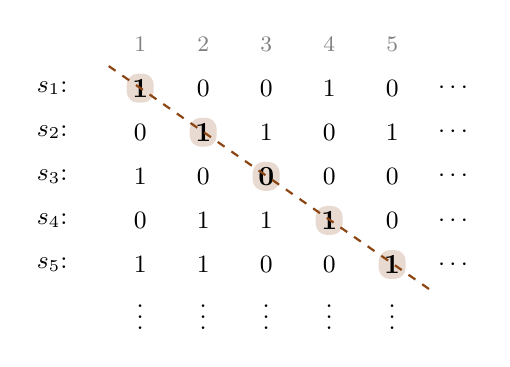
\begin{tikzpicture}[scale=0.8, every node/.style={font=\small}]
    % Header
    \node[font=\footnotesize,gray] at (1.2,1) {1};
    \node[font=\footnotesize,gray] at (2.2,1) {2};
    \node[font=\footnotesize,gray] at (3.2,1) {3};
    \node[font=\footnotesize,gray] at (4.2,1) {4};
    \node[font=\footnotesize,gray] at (5.2,1) {5};
    % Rows
    \node[left] at (0.2,0.3) {$s_1$:};
    \node[left] at (0.2,-0.4) {$s_2$:};
    \node[left] at (0.2,-1.1) {$s_3$:};
    \node[left] at (0.2,-1.8) {$s_4$:};
    \node[left] at (0.2,-2.5) {$s_5$:};
    % Digits
    \node[fill=mAccent!20,rounded corners,inner sep=2pt,font=\bfseries] at (1.2,0.3) {1};
    \node at (2.2,0.3) {0}; \node at (3.2,0.3) {0}; \node at (4.2,0.3) {1}; \node at (5.2,0.3) {0};
    \node at (1.2,-0.4) {0};
    \node[fill=mAccent!20,rounded corners,inner sep=2pt,font=\bfseries] at (2.2,-0.4) {1};
    \node at (3.2,-0.4) {1}; \node at (4.2,-0.4) {0}; \node at (5.2,-0.4) {1};
    \node at (1.2,-1.1) {1}; \node at (2.2,-1.1) {0};
    \node[fill=mAccent!20,rounded corners,inner sep=2pt,font=\bfseries] at (3.2,-1.1) {0};
    \node at (4.2,-1.1) {0}; \node at (5.2,-1.1) {0};
    \node at (1.2,-1.8) {0}; \node at (2.2,-1.8) {1}; \node at (3.2,-1.8) {1};
    \node[fill=mAccent!20,rounded corners,inner sep=2pt,font=\bfseries] at (4.2,-1.8) {1};
    \node at (5.2,-1.8) {0};
    \node at (1.2,-2.5) {1}; \node at (2.2,-2.5) {1}; \node at (3.2,-2.5) {0}; \node at (4.2,-2.5) {0};
    \node[fill=mAccent!20,rounded corners,inner sep=2pt,font=\bfseries] at (5.2,-2.5) {1};
    % Dots
    \node at (6.2,0.3) {$\cdots$};
    \node at (6.2,-0.4) {$\cdots$};
    \node at (6.2,-1.1) {$\cdots$};
    \node at (6.2,-1.8) {$\cdots$};
    \node at (6.2,-2.5) {$\cdots$};
    \node at (1.2,-3.2) {$\vdots$};
    \node at (2.2,-3.2) {$\vdots$};
    \node at (3.2,-3.2) {$\vdots$};
    \node at (4.2,-3.2) {$\vdots$};
    \node at (5.2,-3.2) {$\vdots$};
    % Diagonal line
    \draw[thick, mAccent, dashed] (0.7,0.65) -- (5.8,-2.9);
  \end{tikzpicture}
  \end{center}

  \note{
    The proof uses a clever indirect approach. Rather than trying to show
    directly that no bijection exists, we prove something stronger: every
    countable subset of "A" misses at least one element. To set this up, we
    take any countable subset "E" and arrange its elements in a grid. The
    highlighted diagonal entries are the key to the construction: by looking
    at the "n"-th digit of the "n"-th sequence, we will build a sequence
    that cannot appear anywhere in the list.
  }
\end{frame}

% --- Build 2/3 ---
\begin{frame}{Proof of Theorem 2.14 --- Cantor's Diagonal Argument}
  \begin{proofblock}{Step 2: Construct a new sequence $s$ by flipping the diagonal}
    \begin{itemize}
      \item If the $n$th digit of $s_n$ is $1$, set the $n$th digit of $s$ to $0$
      \item If the $n$th digit of $s_n$ is $0$, set the $n$th digit of $s$ to $1$
    \end{itemize}
  \end{proofblock}

  \vspace{0.3em}
  \begin{hlbox}
    \textbf{From the example:}
    \begin{center}
      \begin{tabular}{r@{\quad}cccccl}
        Diagonal: & $\mathbf{1}$, & $\mathbf{1}$, & $\mathbf{0}$, & $\mathbf{1}$, & $\mathbf{1}$, & $\dots$ \\[2pt]
        $s$:      & $\mathbf{0}$, & $\mathbf{0}$, & $\mathbf{1}$, & $\mathbf{0}$, & $\mathbf{0}$, & $\dots$
      \end{tabular}
    \end{center}

    \vspace{0.3em}
    $s$ differs from $s_n$ in position $n$, so $s \neq s_n$ for every $n$.

    Therefore $\alert{s \notin E}$, yet $s \in A$.
  \end{hlbox}

  \note{
    This is the heart of the argument, and it is worth understanding deeply.
    We only need to change one digit to make "s" different from a given
    sequence, but we need "s" to differ from every sequence in the list
    simultaneously. The diagonal ensures this: by flipping the "n"-th digit
    of "s" sub "n", we guarantee disagreement with "s" sub "n" at position
    "n", regardless of what happens at other positions. No matter how long
    the list is, "s" escapes it. This is why the argument is called the
    diagonal process: the construction literally follows the diagonal of the
    grid. The key insight is that the diagonal touches every row exactly
    once.
  }
\end{frame}

% --- Build 3/3 ---
\begin{frame}{Proof of Theorem 2.14 --- Cantor's Diagonal Argument}
  \begin{proofblock}{Step 3: Conclude}
    Every countable subset $E$ of $A$ is a \emph{proper} subset of $A$.

    \vspace{0.3em}
    If $A$ were countable, then $A$ would be a proper subset of itself --- \alert{contradiction!}

    \vspace{0.3em}
    $\boxed{A \text{ is uncountable.}}$
  \end{proofblock}

  \vspace{0.5em}
  \begin{hlbox}
    \textbf{Connection:} Binary sequences $\longleftrightarrow$ real numbers (binary representation).
    $\Rightarrow$ The set of all real numbers is \alert{uncountable}.
  \end{hlbox}

  \note{
    We have shown that any countable subset of "A" must miss at least one
    element. If "A" itself were countable, it would be a proper subset of
    itself, which is absurd. Therefore "A" is uncountable. This argument is
    called Cantor's diagonal process because the construction follows the
    diagonal of the array. As Rudin notes, if you are familiar with binary
    representations of real numbers, this immediately implies that the real
    numbers are uncountable. We will give a second proof of this fact later,
    in Theorem 2.43.
  }
\end{frame}
}

{
\usebackgroundtemplate{%
  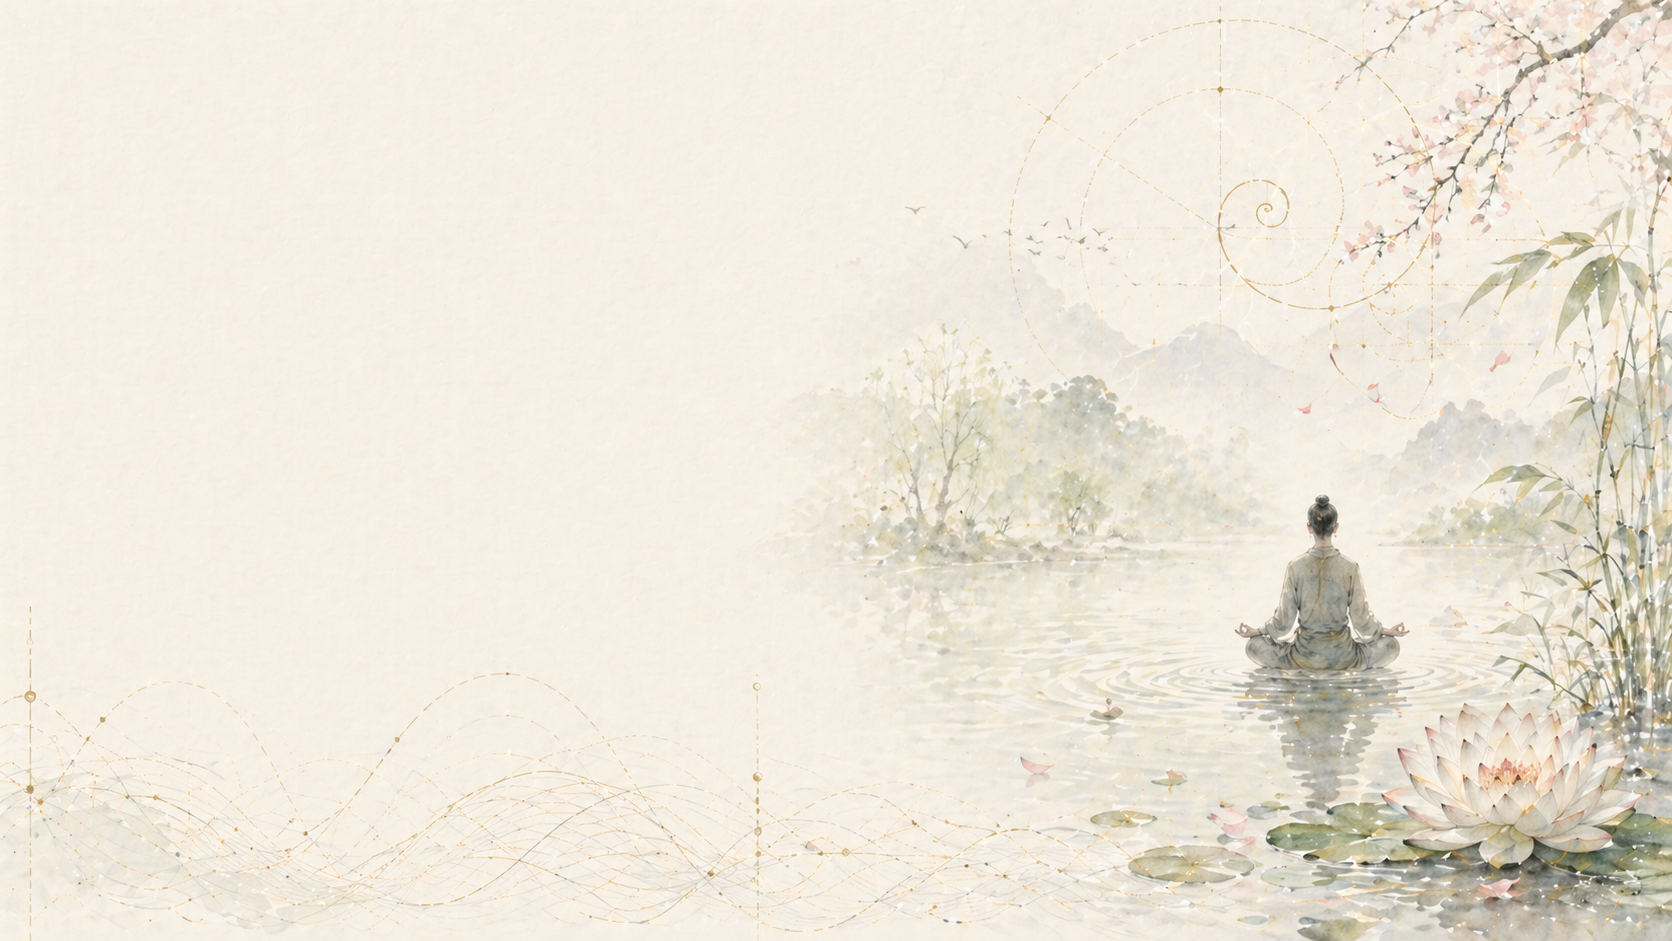
\includegraphics[width=\paperwidth,height=\paperheight,keepaspectratio=false]{chapter_02_bg_06.png}%
}
% ============================================================
\section{Summary}

% ============================================================
% --- Build 1/4 ---
\begin{frame}{Summary}
  \begin{hlbox}
    \textbf{Key takeaways:}
    \begin{itemize}
      \item \textbf{Functions and equivalence:} Two sets have the same size
        ($A \sim B$) iff there is a bijection between them
    \end{itemize}
  \end{hlbox}

  \note{
    Let us review the main ideas from this section. The fundamental concept
    is that of equivalence: two sets are the same size if and only if there
    is a one-to-one correspondence between them.
  }
\end{frame}

% --- Build 2/4 ---
\begin{frame}{Summary}
  \begin{hlbox}
    \textbf{Key takeaways:}
    \begin{itemize}
      \item \textbf{Functions and equivalence:} Two sets have the same size
        ($A \sim B$) iff there is a bijection between them
      \item \textbf{Countable sets:} $\mathbb{Z}$ and $\mathbb{Q}$ are countable;
        countable unions of countable sets remain countable (Theorems 2.12, 2.13)
    \end{itemize}
  \end{hlbox}

  \note{
    The integers and rationals are both countable, which may be surprising
    given how much "denser" the rationals are on the number line. The key
    tools were the diagonal enumeration of Theorem 2.12 and the inductive
    argument of Theorem 2.13. These will be used repeatedly in later
    chapters.
  }
\end{frame}

% --- Build 3/4 ---
\begin{frame}{Summary}
  \begin{hlbox}
    \textbf{Key takeaways:}
    \begin{itemize}
      \item \textbf{Functions and equivalence:} Two sets have the same size
        ($A \sim B$) iff there is a bijection between them
      \item \textbf{Countable sets:} $\mathbb{Z}$ and $\mathbb{Q}$ are countable;
        countable unions of countable sets remain countable (Theorems 2.12, 2.13)
      \item \textbf{Uncountable sets exist:} The set of all binary sequences is
        uncountable (Cantor's diagonal argument, Theorem 2.14)
    \end{itemize}
  \end{hlbox}

  \note{
    But not all infinite sets are countable. Cantor's diagonal argument
    reveals that the set of binary sequences, and therefore the real
    numbers, is strictly larger than countable. This is a profound result:
    it means there are fundamentally different sizes of infinity, and the
    reals represent a bigger infinity than the integers or rationals.
  }
\end{frame}

% --- Build 4/4 ---
\begin{frame}{Summary}
  \begin{hlbox}
    \textbf{Key takeaways:}
    \begin{itemize}
      \item \textbf{Functions and equivalence:} Two sets have the same size
        ($A \sim B$) iff there is a bijection between them
      \item \textbf{Countable sets:} $\mathbb{Z}$ and $\mathbb{Q}$ are countable;
        countable unions of countable sets remain countable (Theorems 2.12, 2.13)
      \item \textbf{Uncountable sets exist:} The set of all binary sequences is
        uncountable (Cantor's diagonal argument, Theorem 2.14)
      \item \textbf{Set operations:} Union, intersection, and their algebraic properties
        (Remarks 2.11)
    \end{itemize}
  \end{hlbox}

  \vspace{0.5em}
  \begin{center}
    \hl{\textbf{Coming up next:} Metric Spaces --- adding the concept of \emph{distance} to sets.}
  \end{center}

  \note{
    We also established the basic algebraic properties of unions and
    intersections, which will be used constantly throughout the rest of the
    book. In the next section, we introduce metric spaces, where we add the
    concept of distance. This will allow us to talk about neighborhoods,
    limits, and open and closed sets, which are the core of topology. Thank
    you for watching, and see you in the next episode.
  }
\end{frame}
}

\end{document}
